% This must be in the first 5 lines to tell arXiv to use pdfLaTeX, which is strongly recommended.
\pdfoutput=1
% In particular, the hyperref package requires pdfLaTeX in order to break URLs across lines.

\documentclass[11pt]{article}

% Remove the "guidelines" option to generate the final version.
%\usepackage[guidelines]{nlpreport} % show guidelines
\usepackage[]{nlpreport} % hide guidelines


% Standard package includes
\usepackage{times}
\usepackage{latexsym}

% For proper rendering and hyphenation of words containing Latin characters (including in bib files)
\usepackage[T1]{fontenc}
% For Vietnamese characters
% \usepackage[T5]{fontenc}
% See https://www.latex-project.org/help/documentation/encguide.pdf for other character sets

% This assumes your files are encoded as UTF8
\usepackage[utf8]{inputenc}

% This is not strictly necessary, and may be commented out,
% but it will improve the layout of the manuscript,
% and will typically save some space.
\usepackage{microtype}
\usepackage{graphicx}
\usepackage{hyperref}
\usepackage{amsmath}
\usepackage{mathtools}
\usepackage{multirow}
\usepackage{listings}
\usepackage{xcolor}
\usepackage{booktabs} % for tables






% THE pdfinfo Title AND Author ARE NOT NECESSARY, THEY ARE METADATA FOR THE FINAL PDF FILE
\hypersetup{pdfinfo={
Title={Recurrent Neural Architectures for POS tagging},
Author={Vincenzo Collura, Gianmarco Pappacoda, Anthea Silvia Sasdelli\\}
}}
%\setcounter{secnumdepth}{0}  
 \begin{document}
%
\title{Assignment 1\\
Recurrent Neural Architectures for POS tagging
}
\explanation{\rm Substitute the $\uparrow$ title $\uparrow$ with your project's title, or with Assignment 1 / 2\\ \smallskip}
% subtitle:
\large \explanation{\rm $\downarrow$ Keep only one of the following three  labels  / leave empty for assignments: $\downarrow$\\}

\author{
Vincenzo Collura,
Gianmarco Pappacoda,
\and
Anthea Silvia Sasdelli\\
Master's Degree in Artificial Intelligence, University of Bologna\\
\{ vincenzo.collura2, gianmarco.pappacoda, anthea.sasdelli \}@studio.unibo.it
}
\maketitle


\attention{DO NOT MODIFY THIS TEMPLATE - EXCEPT, OF COURSE FOR TITLE, SUBTITLE AND AUTHORS.\\ IN THE FINAL VERSION, IN THE \LaTeX\ SOURCE REMOVE THE \texttt{guidelines} OPTION FROM  \texttt{$\backslash$usepackage[guidelines]\{nlpreport\}}.
}

\begin{abstract}
%\begin{quote}

\explanation{
The abstract is very brief summary of your report. Try to keep it no longer than 15-20 lines at most. Write your objective, your approach, and your main observations (what are the findings that make this report worthwhile reading?)}

\large Part-Of-Speech (POS) tagging is an important task at the base of more sophisticated NLP tasks. The goal of this brief report is to explore various (Recurrent) Neural architectures to perform POS tagging. The most important distinction with respect to the task at hand is the use of context which is better exploited by neural solutions as opposed to rule-based techniques. One of the most striking observations was the worsened performance of model variants with respect to the baseline model.  \\


%\end{quote}
\end{abstract}

\attention{\textcolor{red}{NOTICE: THIS REPORT'S LENGTH MUST RESPECT THE FOLLOWING PAGE LIMITS: \begin{itemize}
    \item ASSIGNMENT: \textbf{2 PAGES} 
    \item NLP PROJECT OR PROJECT WORK: \textbf{8 PAGES}
    \item COMBINED NLP PROJECT + PW: \textbf{12 PAGES}
\end{itemize}  PLUS LINKS, REFERENCES AND APPENDICES.\\ 
THIS MEANS THAT YOU CANNOT FILL ALL SECTIONS TO MAXIMUM LENGTH. IT ALSO MEANS THAT, QUITE POSSIBLY, YOU WILL HAVE TO LEAVE OUT OF THE REPORT PART OF THE WORK YOU HAVE DONE OR OBSERVATIONS YOU HAVE. THIS IS NORMAL: THE REPORT SHOULD EMPHASIZE WHAT IS MOST SIGNIFICANT, NOTEWORTHY, AND REFER TO THE NOTEBOOK FOR ANYTHING ELSE.\\ 
FOR ANY OTHER ASPECT OF YOUR WORK THAT YOU WOULD LIKE TO EMPHASIZE BUT CANNOT EXPLAIN HERE FOR LACK OF SPACE, FEEL FREE TO ADD COMMENTS IN THE NOTEBOOK.\\ 
INTERESTING TEXT EXAMPLES THAT EXCEED THE MAXIMUM LENGTH OF THE REPORT CAN BE PLACED IN A DEDICATED APPENDIX AFTER THE REFERENCES.}}


\section{Introduction}
\label{sec:introduction}
\attention{MAX 1 COLUMN FOR ASSIGNMENT REPORTS / 2 COLUMNS FOR PROJECT OR PW / 3 FOR COMBINED REPORTS.}

\explanation{
The Introduction is an executive summary, which you can think of as an extended abstract.  Start by writing a brief description of the problem you are tackling and why it is important. (Skip it if this is an assignment report).} 

\explanation{Then give a short overview of known/standard/possible approaches to that problems, if any, and what are their advantages/limitations.} 

\explanation{After that, discuss your approach, and motivate why you follow that approach. If you are drawing inspiration from an existing model, study, paper, textbook example, challenge, \dots, be sure to add all the necessary references~\cite{DBLP:journals/corr/abs-2204-02311,DBLP:conf/acl/LorenzoMN22,DBLP:conf/clef/AnticiBIIGR21,DBLP:conf/ijcai/NakovCHAEBPSM21,DBLP:conf/naacl/RottgerVHP22,DBLP:journals/toit/LippiT16}.\footnote{\href{https://en.wikipedia.org/wiki/The_Muppet_Show}{Add only what is relevant.}}}

\explanation{Next, give a brief summary of your experimental setup: how many experiments did you run on which dataset. Last, make a list of the main results or take-home lessons from your work.}

\attention{HERE AND EVERYWHERE ELSE: ALWAYS KEEP IN MIND THAT, CRUCIALLY, WHATEVER TEXT/CODE/FIGURES/IDEAS/... YOU TAKE FROM ELSEWHERE MUST BE CLEARLY IDENTIFIED AND PROPERLY REFERENCED IN THE REPORT.}

The objective of this assignment is to explore and evaluate (Recurrent) Neural architectures with dense vector representations to perform Part-Of-Speech (POS) Tagging. Both the dataset, architectures and vector representations were provided. The dataset is the Penn Treebank\cite{Marcus1994} which contains a labeled series of words and their POS tags as well as dependencies between words arranged in phrases, documents. 
The data was downloaded and transformed into a suitable format for data inspection. The third column, representing dependencies between words, has been dropped as per instructions. Each word has been associated with its document and its phrase by means of two different identifiers. This allowed the authors to perform an analysis based on the split methods. For the full analysis please refer to the operative material.

% \section{Background}
% \label{sec:background}
% \attention{MAX 2 COLUMNS (3 FOR COMBINED REPORTS). DO NOT INCLUDE SECTION IF NO BACKGROUND NECESSARY. OMIT SECTION IN ASSIGNMENT REPORTS.}

% \explanation{The Background section is where you briefly provide whatever background information on the domain or challenge you're addressing and/or on the techniques/approaches you're using, that (1) you think is necessary for the reader to understand your work and design choices, and (2) is not something that has been explained to you during the NLP course (to be clear: do NOT repeat explanations of things seen in class, we already know that stuff). If you adapt paragraphs from articles, books, online resources, etc: be sure to clarify which parts are yours and which ones aren't.}


\section{System description}
\label{sec:system}
\attention{MAX 1 COLUMN FOR ASSIGNMENT REPORTS / 4 COLUMNS FOR PROJECT OR PW / 6 FOR COMBINED REPORTS.}

\explanation{
Describe the system or systems you have implemented (architectures, pipelines, etc), and used to run your experiments. If you reuse parts of code written by others, be sure to make very clear your original contribution in terms of
\begin{itemize}
    \item architecture: is the architecture your design or did you take it from somewhere else
    \item coding: which parts of code are original or heavily adapted? adapted from existing sources? taken from external sources with minimal adaptations?
\end{itemize}
It is a good idea to add figures to illustrate your pipeline and/or architecture(s)
(see Figure~\ref{fig:architecture})
%
\begin{figure*}
    \centering
    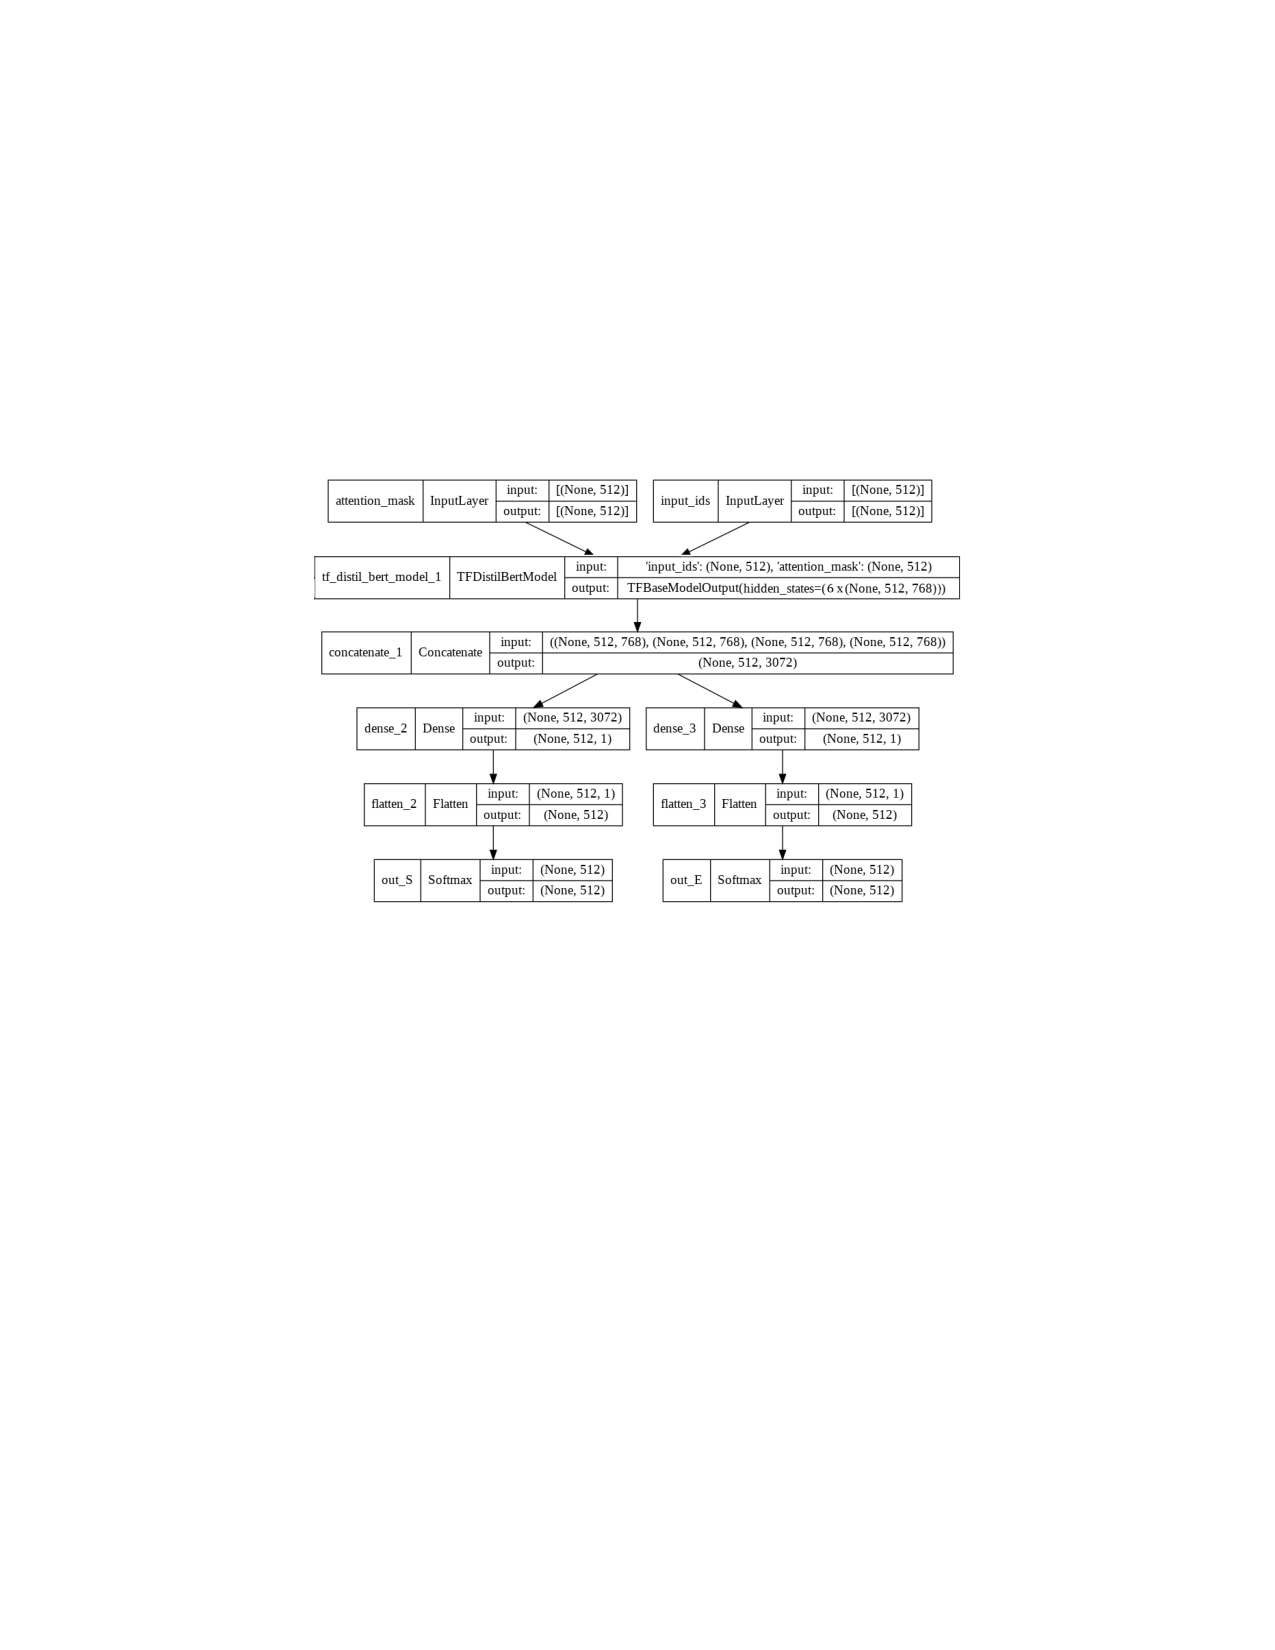
\includegraphics[width=\textwidth]{img/architecture.pdf}
    \caption{Model architecture}
    \label{fig:architecture}
\end{figure*}
}

The implemented system can be roughly divided into three main components:
\begin{itemize}
\item Pre-processing pipeline
\item Word embedding
\item Neural architecture
\end{itemize}

Each subsequent component is dependent on all the previous ones.

The pre-processing pipeline has been purposely kept simple, words have only been converted to lower-case as GloVe\cite{Pennington2014} only has lower-case mappings. Out-Of-Vocabulary (OOV) elements have been dealt with in a rigorous process, the first vocabulary (V1) built started is based on GloVe, then OOV in the training set are computed, a new vocabulary (V2) used for validation purposes only is then created, hence OOV in the validation set are computed, the resulting vocabulary (V3) is then used for testing purposes. A final vocabulary (V4) is computed from the test set.

The word embedding has been implemented as part of the neural network in the form of a static (non-trainable) layer. The embedding layer depends on the building process of the embedding matrix which in turn depends on the vocabulary. During this step words whose embedding is known are translated, words whose embedding is not known (OOVs) are translated into vectors whose dimensions have a uniform distribution. This is due to the fact a hard requirement was imposed, embeddings couldn't be learned or be dynamically dependent on context.

Finally, the following architectures have been tested, all of them start with the aforementioned embedding layer:
\begin{itemize}
\item[] \textbf{Baseline:} a bidirectional LSTM layer followed by a Time-distributed Fully-Connected (Dense) layer with softmax activation.
\item[] \textbf{GRU:} the same architecture as baseline, with GRU units instead of LSTM.
\item[] \textbf{TwoLSTM:} the same architecture as baseline, with an additional bidirectional LSTM layer on top of the first one.
\item[] \textbf{TwoDense:} the same architecture as baseline, with an additional (non-distributed) dense layer at the end, before the softmax activation. In this case the Time-distributed Dense layer has three times the units of the last added layer as to avoid two mirrored layers.
\end{itemize}


%\section{Data}
%\label{sec:data}
%\attention{MAX 2 COLUMNS / 3 FOR COMBINED REPORTS. OMIT SECTION IN ASSIGNMENT REPORTS.}
%
%\explanation{Provide a brief description of your data including some statistics and pointers (references to articles/URLs) to be used to obtain the data. Describe any pre-processing work you did. Links to datasets must be placed later in Section~\ref{sec:links}.}

\section{Experimental setup and results}
\label{sec:results}
\attention{MAX 1 COLUMN FOR ASSIGNMENT REPORTS / 3 COLUMNS FOR PROJECT OR PW / 5 FOR COMBINED REPORTS.}

\explanation{
Describe how you set up your experiments: which architectures/configurations you used, which hyper-parameters and what methods used to set them, which optimizers, metrics, etc.
\\
Then, \textbf{use tables} to summarize your your findings (numerical results) in validation and test. If you don't have experience with tables in \LaTeX, you might want to use \href{https://www.tablesgenerator.com/}{\LaTeX table generator} to quickly create a table template.
}

A seed has been set for all the involved frameworks as to ensure reproducibility.  The dataset was split phrase-wise rather than document-wise as a quick iteration through the baseline model confirmed the authors' intuition of models performing better with phrases contexts rather than document ones. The dataset has been then split into three sets: training, validation, test.

Each neural network has been trained using early stopping, model checkpointing and adaptive learning rate. The chosen optimizer is Nadam (Adam with Nesterov Momentum) as it should provide a faster convergence\cite{Dozat2016}. The main hyperparameter is the number of units in the GRU/LSTM layer. After several attempts authors deemed 100 to be a suitable amount for all the subsequent experiments. For a comprehensive list of hyperparameters, please refer to the operative material.

The selected metric to evaluate the models is the F1-score (rounded 4 digits) excluding punctuation classes. The results of the experiments are shown below.

\begin{table}[]
\centering
\begin{tabular}{@{}lll@{}}
\toprule
         & Validation F1 & Test F1 \\ \midrule
baseline & 0.6998        & 0.7810  \\ \midrule
GRU      & 0.6797        & 0.7657  \\ \midrule
twoLSTM  & 0.6356        & 0.6790  \\ \midrule
twodense & 0.6243        & 0.7284  \\ \bottomrule
\end{tabular}
\end{table}

Notice the test F1 score was calculated for all models, but only the two best models (according to validation F1) should be accounted for.

\section{Discussion}
\label{sec:discussion}
\attention{MAX 1.5 COLUMNS FOR ASSIGNMENT REPORTS / 3 COLUMNS FOR PROJECT / 4 FOR COMBINED REPORTS. ADDITIONAL EXAMPLES COULD BE PLACED IN AN APPENDIX AFTER THE REFERENCES IF THEY DO NOT FIT HERE.}


\explanation{
Here you should make your analysis of the results you obtained in your experiments. Your discussion should be structured in two parts: 
\begin{itemize}
    \item discussion of quantitative results (based on the metrics you have identified earlier; compare with baselines);
    \item error analysis: show some examples of odd/wrong/unwanted  outputs; reason about why you are getting those results, elaborate on what could/should be changed in future developments of this work.
\end{itemize}
}

The two best models are \textit{baseline} and \textit{GRU}. Surprisingly the number of parameters did not translate into a direct performance improvement, on the contrary the most complex models actually performed worse than the most simple ones. The difference in performance between baseline and GRU is negligible while GRU uses $\approx 23.5\%$ less parameters.

Most of the models errors involve nouns (single/plural, common/proper), adjectives and verbs (especially in past tense/past participle). These errors are relevant and can be addressed through a many different approaches, either based on feature engineering or more neural-oriented.

\section{Conclusion}
\label{sec:conclusion}
\attention{MAX 1 COLUMN.}

\explanation{
In one or two paragraphs, recap your work and main results.
What did you observe? 
Did all go according to expectations? 
Was there anything surprising or worthwhile mentioning?
After that, discuss the main limitations of the solution you have implemented, and indicate promising directions for future improvement.
}

It has been possible to implement and evaluate all the models proposed in While bigger models should give better results, the sheer amount of parameters is not indicative of model performance, the baseline model being the most performant while being the simplest among the proposed models. Architecture is actually more important than the amount of stacked layers.

The preprocessing pipeline, albeit short, is actually very important yet the use of GloVe embedding compensate for such absence. As a possible improvement, enriching the pipeline by handling common OOV cases such as dashed-words or numbers in the dataset may improve models' performance.



%\section{Links to external resources}
%\label{sec:links}
%\attention{THIS SECTION IS OPTIONAL}
%\explanation{
%Insert here:
%\begin{itemize}
%    \item a link to your GitHub or any other public repo where one can find your code (only if you did not submit your code on Virtuale); 
%    \item a link to your dataset (only for non-standard projects or project works).
%\end{itemize}
%}

\attention{DO NOT INSERT CODE IN THIS REPORT}

\bibliography{nlpreport.bib}
\end{document}